\section{Non-parametric regression}
\subsection{Gaussian Kernel}
\vspace{-10pt}
\begin{figure}[H]
    \centering
    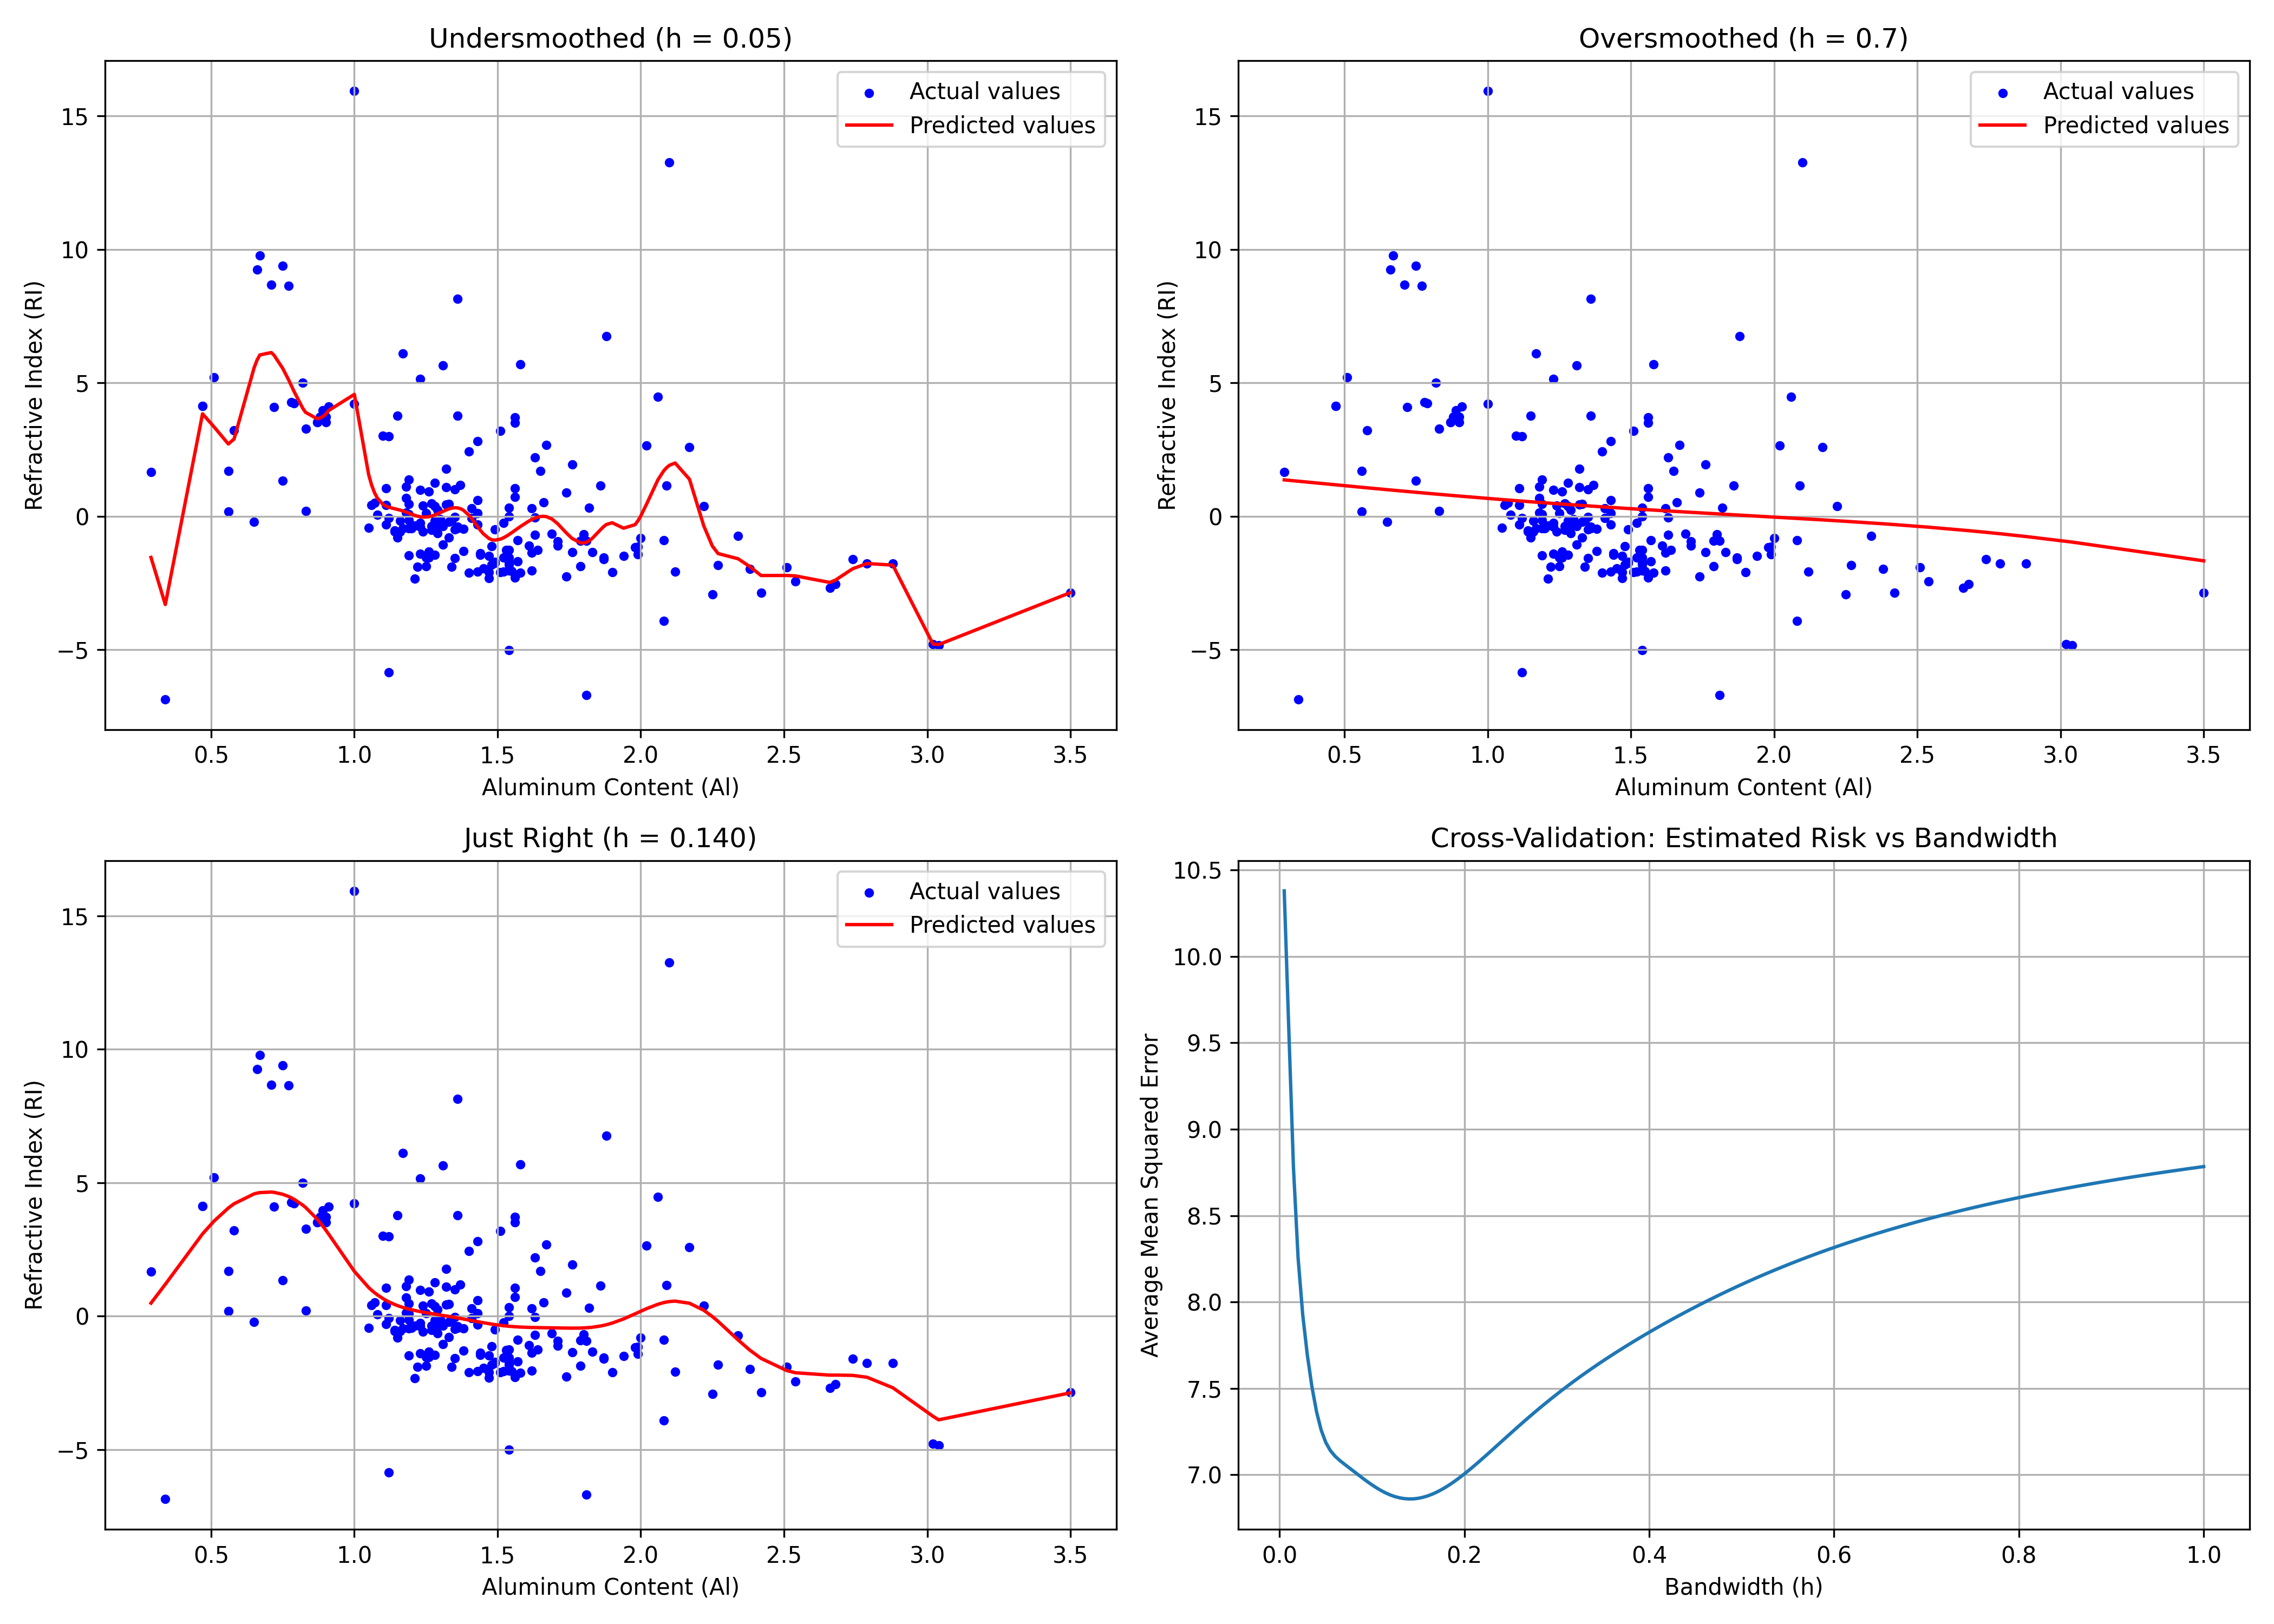
\includegraphics[width=0.5\textwidth]{./images/4/gaussian_kernel_regression.png}
    \caption{Gaussian Kernel Regression}
\end{figure}
The bandwidth corresponding to the minimum estimated risk for the Gaussian kernel is h = 0.140

\subsection{Epanechnikov Kernel}
\vspace{-10pt}
\begin{figure}[H]
    \centering
    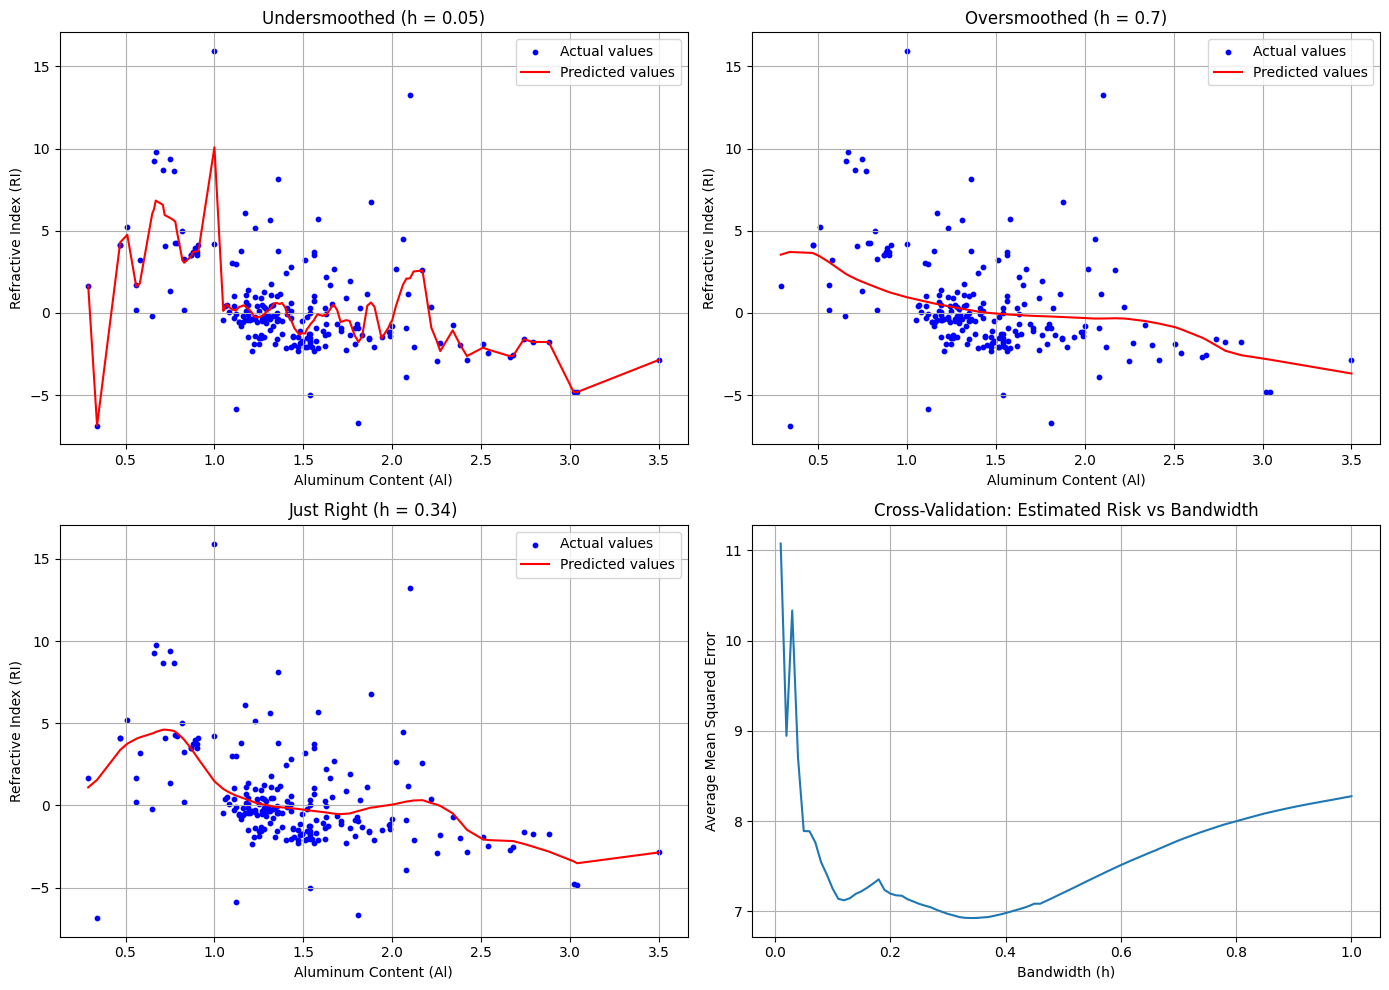
\includegraphics[width=0.5\textwidth]{./images/4/epanechnikov_kernel_regression.png}
    \caption{Epanechnikov Kernel Regression}
\end{figure}
The bandwidth corresponding to the minimum estimated risk for the Epanechnikov kernel is h = 0.325

\subsection{Comments}
The cross validation vs bandwidth for Epanechnikov has multiple local minimas whereas Gaussian has only one.\\
The Gaussian kernel has a lower variance and higher risk compared to the Epanechnikov due to its smoothness.\\
Although the Epanechnikov kernel seems easier to compute, since most powers of $e$ are precomputed in the numpy libraries, the time taken to calculate the Nadaraya Watson estimator is lower for the Gaussian.\\
The estimators look very similar, having almost the same peaks and dips (each Kernel having different bandwidth).\\
The estimators have similar risks as well showing that the dependence on the choice of kernel is not much.